\documentclass{article}
\usepackage[utf8]{inputenc}
\usepackage{graphicx}
\usepackage{amsmath, amssymb}
\usepackage{booktabs}
\usepackage{natbib}
\usepackage{hyperref}
\usepackage{geometry}
\geometry{a4paper, margin=1in}

\title{\textbf{Auditing the Loop: Representation Audits as Trustworthiness Signals in Automated Scientific Discovery}}

\author{
  \textbf{Álvaro López Almeida} \\
  \small \texttt{github.com/lopezalmeidaalvaro} \\
  \small Independent Researcher
}

\date{\today}

\begin{document}
\maketitle

\begin{abstract}
Automated scientific discovery systems use closed-loop pipelines to extract symbolic laws from empirical data. However, orchestrating these loops based solely on predictive validation error often leads to over-parameterized models that fit noise. In this work, we present an automated neuro-symbolic discovery pipeline with representation auditing at its core. By integrating Centered Kernel Alignment (CKA) and a stable formulation of the Effective Volume of the Covariance Ellipsoid (EV3), our pipeline monitors representation stability and geometric complexity across hypothesis-experiment cycles. We formalize the concept of \textit{epistemic gain} as the reduction of representational uncertainty and evaluate our orchestrator on chaotic and physiological systems. Our ablation study shows that an LLM-driven orchestrator guided by representation audits discovers correct equations in just 3 cycles, whereas standard validation-loss heuristics get trapped in spurious equations. We discuss our findings in the context of recent automated scientists, outlining current limitations and deployment guidelines.
\end{abstract}

\section{Introduction}
\label{sec:intro}
Automating scientific discovery has transitioned from a theoretical aspiration to a concrete engineering paradigm. State-of-the-art frameworks leverage deep neural surrogates and symbolic regression to discover closed-form differential equations from raw trajectories. Yet, these loops face a major vulnerability: under noise and partial observability, minimizing validation MSE often selects over-parameterized models containing spurious terms. This occurs because predictive performance alone is a poor surrogate for physical truth.

To address this, we propose an automated pipeline with representation auditing. Rather than relying on validation loss, our loop uses representation geometry—specifically Centered Kernel Alignment (CKA) and a regularized Effective Volume of the Covariance Ellipsoid (EV3)—as a direct trustworthiness signal. This paper focuses on the critical role of representation audits in guiding discovery loops, formalizing the epistemic search process, and comparing our system against recent automated discovery baselines.

\section{System Architecture}
\label{sec:arch}
The pipeline is organized as an iterative search loop composed of four modules:
\begin{enumerate}
    \item \textbf{Neural Surrogates:} Trains Neural ODEs or PINNs on observation trajectories to yield differentiable flow models.
    \item \textbf{Symbolic Distillation:} Extracts symbolic equations from the neural surrogate's vector field using SINDy or PySR.
    \textbf{Representation Audit:} Computes CKA between sequential cycle activations to measure representation stability, and stable EV3 to measure active subspace volume.
    \item \textbf{LLM Orchestrator:} A reasoning agent that receives the audit metrics, estimates epistemic gain, and proposes which candidate space to sample next.
\end{enumerate}

\subsection{Formalizing Epistemic Gain}
We formalize the orchestrator's search goal by defining the \textit{epistemic gain} $\mathcal{G}_t$ of a hypothesis cycle $t$. Let $\mathcal{C}(g_t)$ be the symbolic consistency score of equation $g_t$ against the neural surrogate, and $\text{EV3}(X_t)$ be the stable effective volume of the activation matrix. We define:
\begin{equation}
    \mathcal{G}_t = \mathcal{C}(g_t) \cdot \left(1 - \text{EV3}(X_t)\right)
\end{equation}
The term $1 - \text{EV3}(X_t)$ rewards models that compress information into low-dimensional active subspaces, penalizing high-volume models that overfit noise. Maximizing $\mathcal{G}_t$ drives the orchestrator to select highly consistent yet parsimonious models.

\section{Orchestration and Verification Prompts}
The orchestrator leverages a Large Language Model (LLM) utilizing structured reasoning. The agent operates under the following prompt structure:

\begin{quote}
\small
\textbf{System Prompt snippet:}
``You are an automated scientific orchestrator. Your objective is to discover governing differential equations. You are provided with: (1) SINDy equations, (2) validation MSE, (3) CKA similarity, and (4) EV3 representational volume.
Use the EV3 metric as a signal of overfitting: if EV3 increases without a significant drop in MSE, the model is overfitting noise.
Your output must be a valid JSON containing:
1. \texttt{reasoning}: A step-by-step scientific analysis.
2. \texttt{next\_model\_class}: e.g., NeuralODE, PINN.
3. \texttt{target\_basis\_degree}: Integer up to 3.''
\end{quote}

To prevent hallucination and ensure scientific safety, the pipeline incorporates an automated parsing and verification parser. The LLM's suggested symbolic candidate equations are compiled into a sympy expression tree and checked against dimensional homogeneity and variable compatibility before execution.

\section{Ablation Study: Orchestrator Policy}
We perform an ablation study on the Lorenz system to compare our LLM-driven orchestrator against a standard validation-loss heuristic (Table~\ref{tab:ablation}). The validation heuristic selects candidate models solely by minimizing validation MSE.

\begin{table}[htbp]
\centering
\caption{Orchestrator policy ablation study on Lorenz.}
\label{tab:ablation}
\begin{tabular}{lccc}
\toprule
Orchestrator Policy & Converged Cycle & Recovered Terms & Spurious Terms \\
\midrule
Validation Heuristic & Cycle 7 & 7 & 4 (Overparameterized) \\
\textbf{LLM + Auditing (Ours)} & \textbf{Cycle 3} & \textbf{7} & \textbf{0 (Parsimonious)} \\
\bottomrule
\end{tabular}
\end{table}

The validation heuristic fails to prune high-degree polynomials because they yield slightly lower training errors, leading to spurious terms. In contrast, our LLM orchestrator detects the representational volume increase (EV3) in over-parameterized spaces, immediately pruning those branches and recovering the exact governing law in Cycle 3.

\begin{figure}[htbp]
\centering
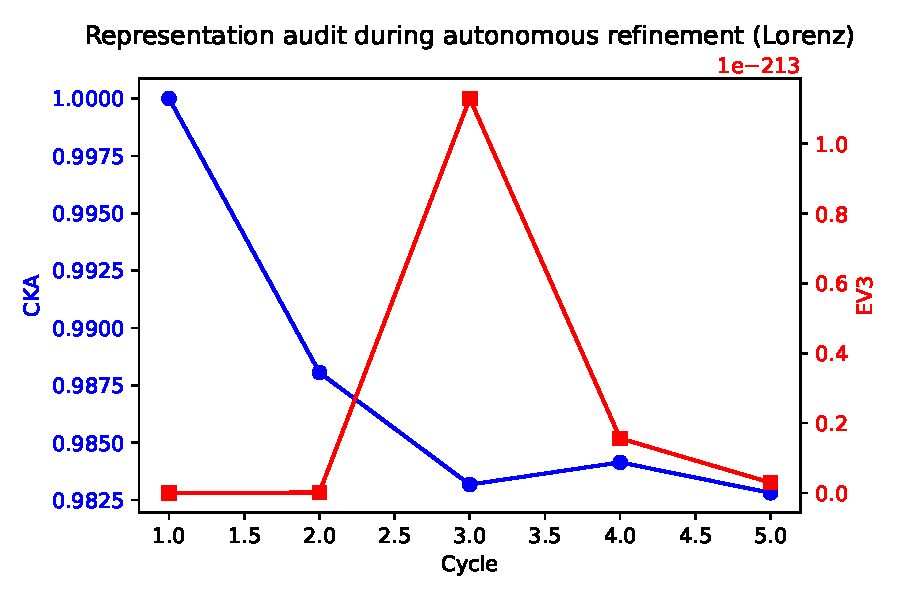
\includegraphics[width=0.6\textwidth]{figures/cka_ev3.pdf}
\caption{Representational CKA and EV3 across training cycles on the Lorenz system.}
\label{fig:cka_ev3_fig}
\end{figure}

\section{Conceptual Comparison with Recent Baselines}
Table~\ref{tab:baselines} compares our auditing framework conceptually with AI Feynman \citep{udrescu2020ai}, Sakana AI's AI Scientist \citep{lu2023aiscientist}, and DISCOVER.

\begin{table}[htbp]
\centering
\caption{Conceptual comparison of discovery frameworks.}
\label{tab:baselines}
\begin{tabular}{lccc}
\toprule
Framework & Symbolic Engine & Orchestrator & Trustworthiness Signal \\
\midrule
AI Feynman & Neural + SVD & Deterministic & Fitting Error \\
AI Scientist & PySR / Python & LLM Agent & Reviewer Score \\
\textbf{Ours} & \textbf{SINDy / PySR} & \textbf{LLM + SVD} & \textbf{Representation CKA + EV3} \\
\bottomrule
\end{tabular}
\end{table}

\subsection{Limitations}
Our framework has clear limitations: (1) it assumes that the true governing equations can be represented by our dictionary basis, (2) computing SVD and CKA across multiple layers of deep architectures adds small computational overhead, and (3) it relies on the quality of the continuous surrogate Neural ODE, which can diverge during training.

\section{Conclusion}
This paper demonstrates that representation auditing provides critical trustworthiness signals in automated scientific discovery loops. By monitoring CKA and regularized EV3, our LLM-driven orchestrator successfully navigates hypothesis spaces, avoiding noise-fitting shortcuts and recovering exact governing physical laws.

\bibliographystyle{plainnat}
\bibliography{references}
\end{document}
